\chapter{Data Analysis and Results}\label{result}

Here the results of the tests are presented. First, the parameters detected using PoLaR BEAR and BEAR are shown and compared to the true parameters. Second, the difference between the detections and the true parameters are observed, and the accuracy of the outputs of PoLaR BEAR and BEAR are compared to characterize the performance of PoLaR BEAR. 

\section{Real FRB data}

PoLaR BEAR was able to detect all 19 FRBs in all real FRB files. As a comparison, the original BEAR was only able to detect 14 out of 19 FRBs. The non-detections were from FRB 130729, FRB 140514, and the three FRB 200428 data due to small pulse widths, relatively low SNR, and updated header formatting respectively, for which the latter was easily overcome in PoLaR BEAR by adding them to the dictionary. The detected DM, W, and SNR for PoLaR BEAR and BEAR for each of the real FRBs are as shown in Table \ref{tab:frbres}.

\begin{table}
    \centering
    \caption[Detection results for real FRB data]{Detection results for real FRB data using PoLaR BEAR and BEAR.}
    \tiny
    \def\arraystretch{1.25}
    \begin{tabular}{cccccccccc}
        \hline
             FRB     &  True DM  &  PoLaR DM  &  BEAR DM  &  True  &  PoLaR  &  BEAR  &  True  &  PoLaR  &  BEAR  \\
             & ($\cmp$) & ($\cmp$) & ($\cmp$) & W (ms) & W (ms) & W (ms) & SNR & SNR & SNR \\
        \hline
         FRB 010124  &   790.3   &       790       &  790.238  &   10.6   &      7.5       &  11.25   &    10.6    &      22.53       &  23.0684   \\
         FRB 010621  &    745    &       748       &  749.395  &    7     &       10       &   7.5    &    16.3    &     15.7427      &  16.1699   \\
         FRB 010724  &    375    &       374       &  930.767  &    20    &       24       &   1529   &    100     &     34.4823      &  50.6785   \\
         FRB 090625  &  899.55   &       899       &  899.889  &   1.92   &      2.56      &   1.92   &     30     &     23.9272      &  24.1128   \\
         FRB 110220  &  944.38   &       946       &  944.635  &   6.59   &      6.4       &   5.76   &     54     &     31.1559      &  34.5971   \\
         FRB 110626  &    723    &       724       &  721.413  &   1.41   &      2.56      &   1.92   &     12     &     9.17705      &  9.43211   \\
         FRB 110703  &  1103.6   &      1105       &  1106.37  &   3.9    &      3.84      &   3.2    &     17     &     15.0202      &   14.646   \\
         FRB 120127  &   553.3   &       554       &  555.683  &   1.21   &      1.28      &   1.92   &     13     &     9.80996      &  11.2739   \\
         FRB 121002  &  1629.18  &      1630       &  1630.05  &   5.44   &      6.4       &   5.76   &     16     &     14.4355      &  15.4915   \\
         FRB 130626  &   952.4   &       953       &  953.381  &   1.98   &      2.56      &   1.92   &     21     &     14.8354      &  16.5966   \\
         FRB 130628  &  469.88   &       471       &  469.444  &   0.64   &      1.28      &   1.28   &     29     &     15.7191      &  16.5475   \\
         FRB 130729  &    861    &       854       &     -     &  15.61   &      6.4       &    -     &     14     &     8.30313      &     -      \\
         FRB 140514  &   561.7   &       562       &     -     &  2.816   &      3.84      &    -     &     16     &     8.14297      &     -      \\
         FRB 150215  &  1105.6   &      1107       &  1106.37  &   2.88   &      2.56      &   3.2    &     19     &     14.2704      &  14.5193   \\
         FRB 121102  &    557    &       579       &    584    &    3     &      5.12      &   5.12   &     14     &     22.1387      &  27.9405   \\
         FRB 200428a &  337.702  &       335       &     -     &   0.61   &    1.31072     &    -     &     20     &     10.5442      &     -      \\
         FRB 200428b &  337.702  &       332       &     -     &   0.61   &    1.31072     &    -     &     15     &     10.4817      &     -      \\
         FRB 200428c &  337.702  &       335       &     -     &   0.61   &    1.31072     &    -     &     21     &     8.37221      &     -      \\
        \hline
    \end{tabular}
    \label{tab:frbres}
\end{table}

\section{Generated FRB data}

PoLaR BEAR was able to detect 49 out of 50 FRBs in our sample of fake FRB data. Similarly, the original BEAR was also able to detect 49 out of 50 FRBs. Both programs were not able to detect Fake 19, which has one of the lowest SNR at 9.00864. The detected DM, W, and SNR for PoLaR BEAR and BEAR for each of the fake FRBs are as shown in Table \ref{tab:fakeres}.

\begin{table}
    \centering
    \caption[Detection results for fake FRB data]{Detection results for Fake FRB data using PoLaR BEAR and BEAR.}
    \tiny
    \def\arraystretch{1.25}
    \begin{tabular}{cccccccccc}
    \hline
      Fake  &  True DM  &  PoLaR DM  &  BEAR  &  True  &  PoLaR   &  BEAR  &  True  &  PoLaR  &  BEAR  \\
      & ($\cmp$) & ($\cmp$) & ($\cmp$) & W (ms) & W (ms) & W (ms) & SNR & SNR & SNR \\
    \hline
       1   &  566.158  &       563       &  565.451  & 3.47103  &      3.84      &   3.2    &  34.1301   &     31.3015      &  32.3983   \\
       2   &  1476.21  &      1478       &  1476.53  & 3.97177  &      3.84      &   3.2    &  46.3679   &     40.6662      &  40.4863   \\
       3   &  1858.64  &      1858       &  1861.15  & 2.57209  &      2.56      &   3.2    &  26.5634   &     23.8261      &  24.5231   \\
       4   &  399.97   &       397       &  396.604  & 2.77513  &      2.56      &   3.2    &  10.1587   &     8.70667      &  8.97403   \\
       5   &  573.649  &       573       &  572.429  & 0.710951 &      1.28      &   1.28   &  16.1083   &     10.5715      &  11.0524   \\
       6   &  1187.42  &      1188       &  1187.81  &  3.8433  &      3.84      &   3.2    &  34.5618   &     29.9834      &  30.1843   \\
       7   &  1028.33  &      1027       &  1028.99  & 1.66997  &      2.56      &   1.92   &  42.8729   &     33.8904      &  38.1275   \\
       8   &  1337.1   &      1340       &  1339.68  & 3.16891  &      3.84      &   3.2    &  45.5356   &     37.8317      &   40.721   \\
       9   &  1364.17  &      1361       &  1363.64  & 2.16554  &      2.56      &   1.92   &  15.2655   &     12.5744      &  14.0023   \\
      10   &  1321.39  &      1321       &  1319.68  & 4.92548  &      6.4       &   5.76   &  33.4504   &     29.5878      &  31.4454   \\
      11   &  1666.28  &      1667       &  1665.35  & 3.77166  &      3.84      &   3.2    &  44.4121   &     39.6793      &  40.3442   \\
      12   &  728.46   &       725       &  729.275  & 2.61624  &      2.56      &   3.2    &  20.7568   &     17.2411      &  18.0443   \\
      13   &  789.509  &       786       &  789.231  & 1.77699  &      2.56      &   1.92   &  44.6985   &     34.3899      &  39.4427   \\
      14   &  1744.95  &      1742       &  1744.26  & 4.58435  &      3.84      &   5.76   &  37.8006   &     33.5477      &  35.5756   \\
      15   &  1530.5   &      1529       &  1529.48  & 1.14656  &      1.28      &   1.28   &  47.1532   &     33.9406      &  37.9887   \\
      16   &  742.392  &       744       &  747.275  & 3.77817  &      3.84      &   3.2    &  26.9581   &     23.4275      &  23.8539   \\
      17   &  1504.54  &      1508       &  1509.51  & 3.39606  &      3.84      &   3.2    &   9.8772   &     8.65455      &  9.25259   \\
      18   &  669.927  &       671       &  666.341  & 2.79792  &      3.84      &   3.2    &  11.7874   &      9.7949      &  10.5248   \\
      19   &  1287.46  &        -        &     -     & 1.60874  &       -        &    -     &  9.00864   &        -         &     -      \\
      20   &  669.849  &       668       &  667.341  & 3.16439  &      2.56      &   3.2    &  23.6871   &      21.886      &   22.934   \\
      21   &  1395.44  &      1397       &  1396.62  & 4.48013  &      3.84      &   5.76   &  39.7673   &     35.3169      &   35.334   \\
      22   &  678.089  &       679       &  679.341  & 2.73084  &      2.56      &   3.2    &  21.4789   &      17.189      &  17.5459   \\
      23   &  393.089  &       398       &  396.604  & 2.40809  &      2.56      &   1.92   &  35.0218   &     27.1215      &  29.6006   \\
      24   &  848.94   &       852       &  852.165  &  2.227   &      2.56      &   1.92   &   17.862   &     16.0703      &  29.1919   \\
      25   &  846.969  &       848       &  846.165  & 1.62728  &      1.28      &   1.92   &  33.0218   &     24.5658      &  26.6359   \\
      26   &  1358.91  &      1359       &  1355.66  & 4.79527  &      3.84      &   5.76   &  18.5694   &     17.1126      &  17.8909   \\
      27   &  480.351  &       482       &  480.538  & 2.97478  &      2.56      &   3.2    &  42.4061   &      36.258      &   38.868   \\
      28   &  1668.8   &      1671       &  1670.35  & 2.42997  &      2.56      &   1.92   &  29.9655   &     25.6359      &  25.8296   \\
      29   &  359.856  &       364       &  357.648  &  4.1512  &      3.84      &   3.2    &  31.7901   &     25.3873      &   26.919   \\
      30   &  426.874  &       428       &  427.582  & 1.36033  &      1.28      &   1.28   &  28.9338   &     21.0301      &  24.2949   \\
      31   &  1308.65  &      1311       &  1312.67  & 2.71006  &      3.84      &   3.2    &   11.783   &     10.4659      &   11.039   \\
      32   &  352.708  &       354       &  352.648  & 0.863634 &      1.28      &   1.28   &   28.142   &     18.2329      &  21.6419   \\
      33   &  745.125  &       747       &  747.275  & 0.82552  &      1.28      &   1.28   &   32.431   &     20.4732      &  23.1195   \\
      34   &  1355.43  &      1358       &  1356.66  & 2.69499  &      2.56      &   3.2    &  34.6861   &     28.9677      &  30.6762   \\
      35   &  741.125  &       737       &  741.275  & 2.97293  &      3.84      &   3.2    &  11.9684   &     10.4464      &  11.0272   \\
      36   &  1046.19  &      1047       &  1044.97  & 3.98829  &      3.84      &   3.2    &  18.2477   &     15.8839      &  15.2783   \\
      37   &  1199.7   &      1202       &  1199.81  &  1.4724  &      1.28      &   1.92   &  17.7535   &     13.5037      &  14.4868   \\
      38   &  518.282  &       519       &  517.495  & 4.72503  &      3.84      &   5.76   &   49.626   &     40.4404      &   43.56    \\
      39   &  1799.01  &      1802       &  1796.22  & 4.07805  &      3.84      &   3.2    &  23.5333   &     22.0723      &  21.9321   \\
      40   &  670.819  &       668       &  665.341  & 2.36506  &      2.56      &   3.2    &  19.3561   &      15.944      &   16.13    \\
      41   &  1688.62  &      1686       &  1686.33  & 0.997483 &      1.28      &   1.28   &  40.5665   &     25.9701      &  30.3779   \\
      42   &  1195.6   &      1197       &  1195.81  & 1.85354  &      2.56      &   1.92   &  30.0239   &     23.9527      &  25.8458   \\
      43   &  1869.7   &      1868       &  1868.15  & 1.82071  &      2.56      &   1.92   &  24.1694   &     21.2072      &  21.7146   \\
      44   &  587.108  &       591       &  585.429  & 3.61604  &      3.84      &   3.2    &  11.8553   &     11.8643      &  13.0866   \\
      45   &  601.626  &       604       &  598.407  & 4.16235  &      3.84      &   3.2    &  33.3841   &     29.8459      &  29.7412   \\
      46   &  746.818  &       746       &  744.275  & 2.50385  &      2.56      &   3.2    &  9.14934   &     8.54968      &   8.387    \\
      47   &  1268.11  &      1272       &  1269.75  & 1.02883  &      1.28      &   1.28   &  15.4958   &     10.3593      &  12.6025   \\
      48   &  1818.44  &      1818       &  1818.2   & 4.73783  &      3.84      &   5.76   &  40.2606   &     34.5793      &  36.6491   \\
      49   &  1734.89  &      1734       &  1733.29  &  2.3775  &      2.56      &   3.2    &  40.4545   &     33.3137      &  33.9313   \\
      50   &  917.338  &       915       &  918.099  & 3.38351  &      3.84      &   3.2    &  40.1697   &     33.9579      &   36.37    \\
    \hline
    \end{tabular}
    \label{tab:fakeres}
\end{table}

\section{Difference in detections for PoLaR BEAR and BEAR}

\subsection{Detection DM}

Histograms of the DM difference in detections from PoLaR BEAR and BEAR for real FRB data and fake FRB data are shown in Figure \ref{fig:dmdiff}. The outliers here are defined to be data with DM difference of $\pm 10 \cmp$. For real FRB data, PoLaR BEAR has 1 outlier ($22 \cmp$) whereas BEAR has 2 outliers ($555.77 \cmp$, $27 \cmp$). For fake FRB data, both PoLaR BEAR and BEAR exhibited no outliers, with most detections occuring within $\pm 5 \cmp$. In both cases, it can be seen that PoLaR BEAR performs on par with BEAR, with detections close to the true DM. 

\begin{figure}
    \centering
    \begin{minipage}{0.5\textwidth}
        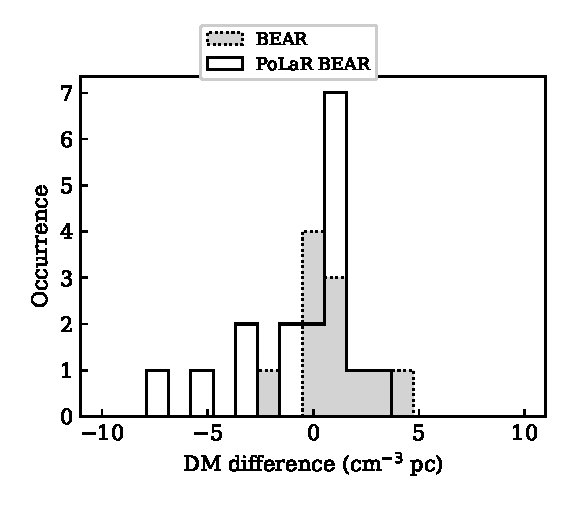
\includegraphics[width=\textwidth]{Graphs/frbdmdiff.eps}
    \end{minipage}%
    \begin{minipage}{0.5\textwidth}
        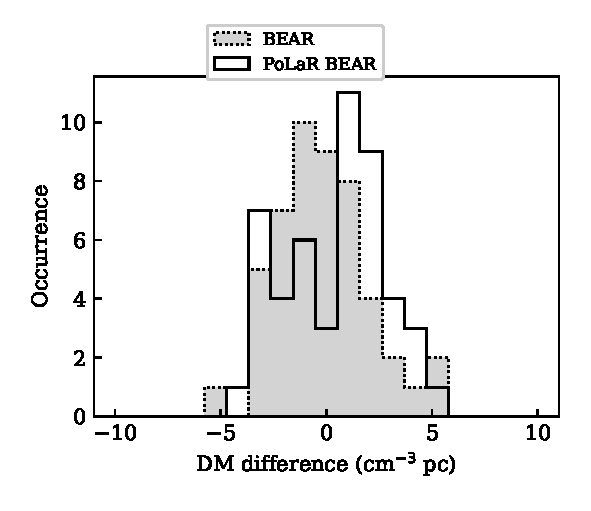
\includegraphics[width=\textwidth]{Graphs/fakedmdiff.eps}
    \end{minipage}
    \caption[Histograms of DM difference]{Histograms of DM difference in detections from PoLaR BEAR and BEAR for real FRB data (left) and fake FRB data (right).}
    \label{fig:dmdiff}
\end{figure}

\subsection{Detection W}

Histograms of the W difference in detections from PoLaR BEAR and BEAR for real FRB data and fake FRB data are shown in Figure \ref{fig:wdiff}. The outliers here are defined to be data with W difference of $\pm 10$ ms. For real FRB data, PoLaR BEAR exhibited no outliers whereas BEAR has 1 outlier ($1509$ ms). For fake FRB data, both PoLaR BEAR and BEAR exhibited no outliers, with most detections occuring within $\pm 2$ ms. It can be seen that for real FRBs, detections from BEAR do have smaller errors whereas PoLaR BEAR reports larger W. On the other hand, for fake FRBs, PoLaR BEAR was much more consistent with much more detections occuring close to the true W.

\begin{figure}
    \centering
    \begin{minipage}{0.5\textwidth}
        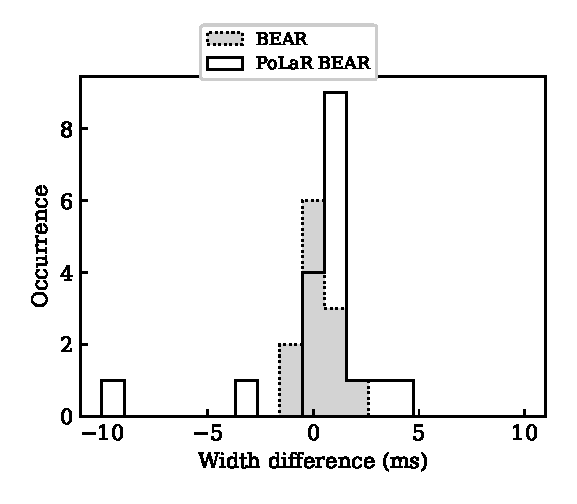
\includegraphics[width=\textwidth]{Graphs/frbwdiff.eps}
    \end{minipage}%
    \begin{minipage}{0.5\textwidth}
        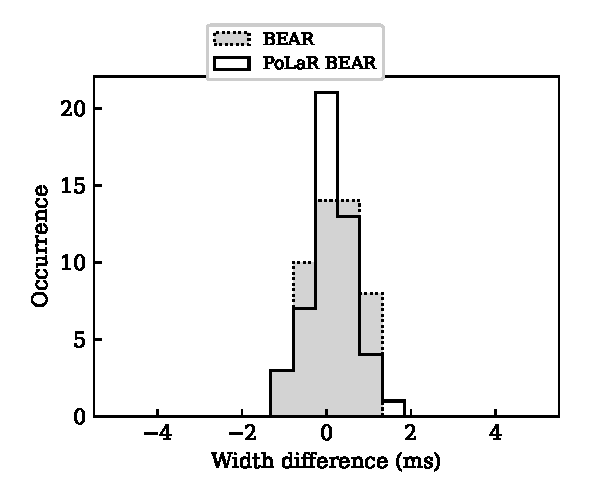
\includegraphics[width=\textwidth]{Graphs/fakewdiff.eps}
    \end{minipage}
    \caption[Histograms of W difference]{Histograms of W difference in detections from PoLaR BEAR and BEAR for real FRB data (left) and fake FRB data (right).}
    \label{fig:wdiff}
\end{figure}

\subsection{Detection SNR}

Histograms of the SNR difference in detections from PoLaR BEAR and BEAR for real FRB data and fake FRB data are shown in Figure \ref{fig:snrdiff}. The outliers here are defined to be data with SNR difference of $\pm 30$. For real FRB data, PoLaR BEAR exhibited no outliers whereas BEAR has 1 outlier ($-49.32$). For fake FRB data, both PoLaR BEAR and BEAR exhibited no outliers, with most detections occuring within $\pm 10$. In both cases, PoLaR BEAR performs as well as BEAR. 

\begin{figure}
    \centering
    \begin{minipage}{0.5\textwidth}
        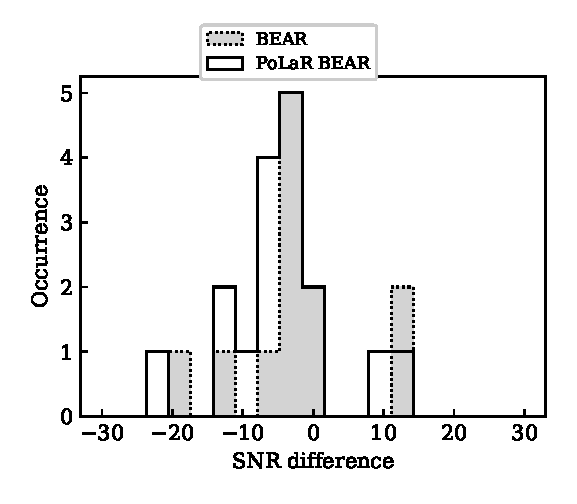
\includegraphics[width=\textwidth]{Graphs/frbsnrdiff.eps}
    \end{minipage}%
    \begin{minipage}{0.5\textwidth}
        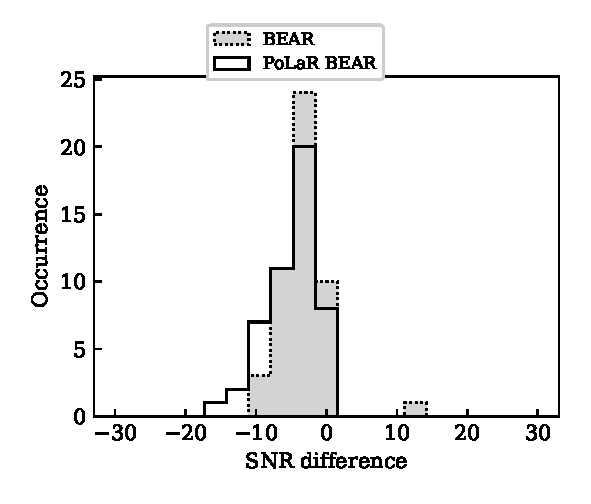
\includegraphics[width=\textwidth]{Graphs/fakesnrdiff.eps}
    \end{minipage}
    \caption[Histograms of SNR difference]{Histograms of SNR difference in detections from PoLaR BEAR and BEAR for real FRB data (left) and fake FRB data (right).}
    \label{fig:snrdiff}
\end{figure}